%\subsection{Neocortical Layer 4/5 Pyramidal Cell Test Suite}

%Direct Quote: "widening of the spike shape, decrease of the firing rate and change in the interspike interval distribution". %All these single unit waveform shapes increased their width with temperature.\cite{goldin2017temperature}



%\subsubsection{%\subsection{Section 2.1}
%
%2. Results for several optimized models.
%    2a. First just do basic ones (like Izhikevich) for a few cell types, then you can close with L5PC.
%    2b. The app (which supports 2a).

%\subsubsection{2a}

\subsubsection{Performance of Layer 5 Pyramidal Neuron Somatosensory model on NeuronUnit tests}
%Hind-limb
\cite{van2016bluepyopt}
%To understand the validity of model re-purposing, we tested a model constrained on Layer 5 Somatosensory cortex Pyramidal neurons. 

Below I introduce a different approach to parameter fitting work: a multi-compartment, conductance based layer 5 pyramidal cell model, was appropriated from BluePyOpt optimization framework, and massaged into the NeuronUnit framework. This model subserved as one of many component neurons in the priginal formulation of the blue brain project \cite{markram2015reconstruction}. This elaborate biophysical model is the philosophical opposite of the reduced models focused on in the majority of this thesis work, since the model incorporates electrically complex phenomena instead of excluding it from the model. The complex model includes a dendritic action potential which can travel "backwards" from distal dendrite to soma where it is free to summate with incomming EPSPs. As you can see in the list of parameters \ref{fig:ca1_parameters}, The model has different adjustable conductance's in 3 out of 4 membrane domains including axons, dendrites, and soma. There are also other parameters (not displayed here) which are fixed, but those specified in \ref{fig:parameters} are amenable to fitting in the context of optimization.

There were two points to this exercise: the first point was to show that multi-compartment conductance based models, are very slow to evaluate, and the second point was, that without enough time, the results are not necessarily the best possible. However, the model itself happens to be a determing factor in reducing time. The resulting optimized model might serve as a useful benchmark, for us to evaluate the relative performance of reduced model fits. 

A suite of neuronunit tests containing the tests: rheobase value, membrane voltage time constant ($tau_{m})$, input resistance was computed. 
% somatosensory cortex, or cell from the l5 somatosensory rat, hind leg region, so it is probably not comparable to NeuroElectro Data.

Significant development work went into making the model eligible to take NeuronUnit tests, and amenable to NeuronUnit driven optimization, to make this complicated conductance based multi-compartment model interoperable with the neuronunit test judging paradigm. The intention is that by making this model inter-operable with NeuronUnit the model will be able to amenable to different, optimization. 

Before optimization:
\begin{figure}
    \centering
    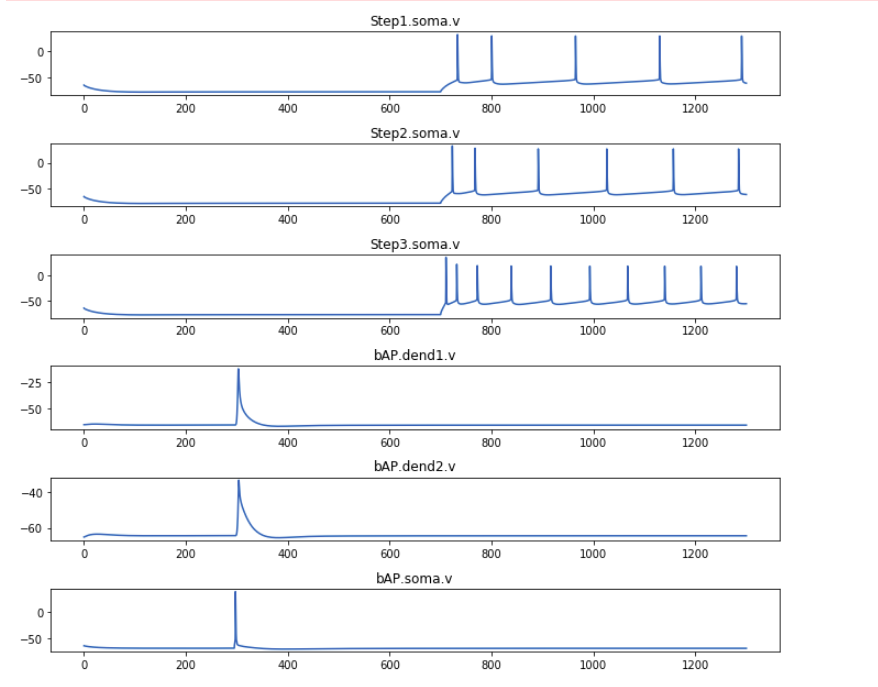
\includegraphics{figures/l5pc_before_opt}
    \caption{Caption}
    \label{fig:my_label}
\end{figure}
After optimization

\begin{figure}
    \centering
    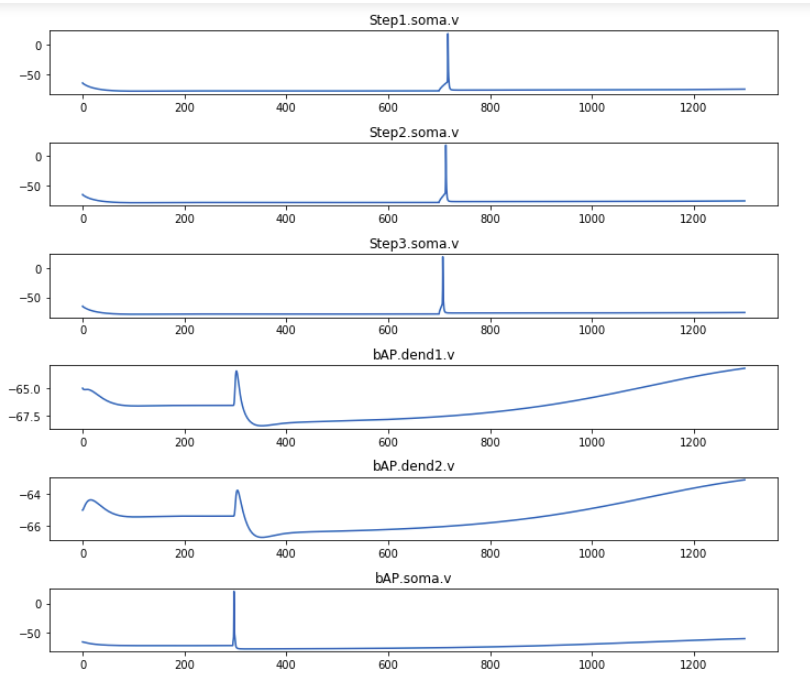
\includegraphics{figures/l5pc}
    \caption{Membrane potential versus time in the layer 5 pyramidal neuron}
    \label{fig:after_optimization}
\end{figure}



\begin{figure}
    \centering
    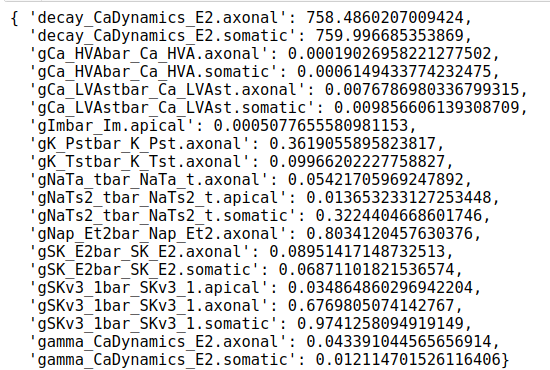
\includegraphics{figures/parameters_opt_l5pc.png}
    \caption{Caption}
    \label{fig:ca1_parameters}
\end{figure}




\begin{figure}
\begin{center}
\centering
\begin{subfigure}%{.2\textwidth}
  \centering
   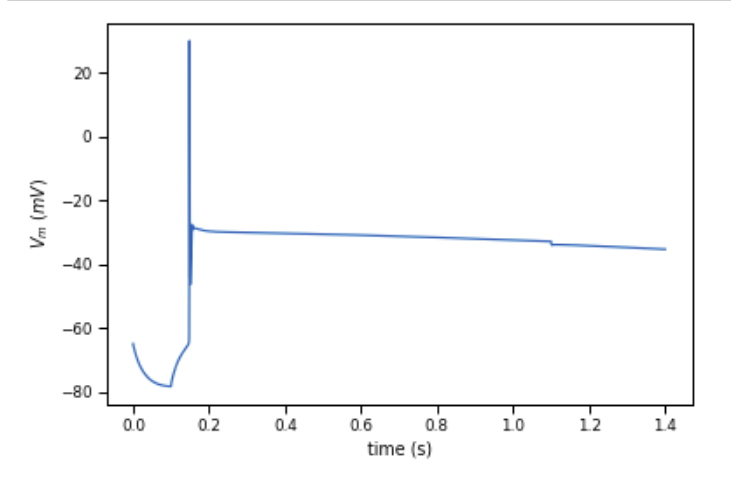
\includegraphics[scale=0.5]{figures/correct_active_l5pc.png}
    \caption{A current injection sufficient for causing a single spike is applied for a whole second from $100ms-1100ms$}
  \label{fig:sub1}
\end{subfigure}

As a reference point for understanding 
    \caption{The spike shape is very brief in duration, and so it is worth zooming in for a closer look}

\centering
\begin{subfigure}%{.2\textwidth}
  \centering
    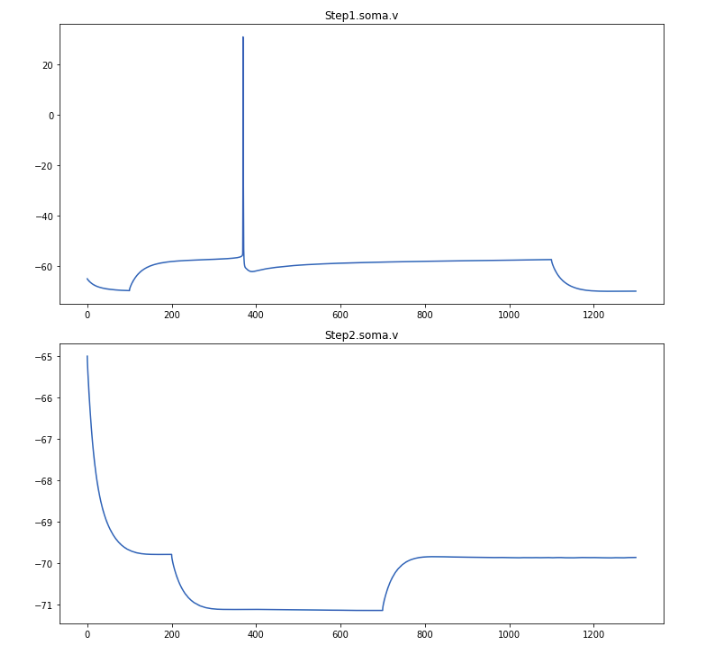
\includegraphics[scale=0.5]{figures/L5Somatosensory_not_optimized.png}
    \caption{$V_{m}$ in $(mV)$ versus time $ms$, plots include a suprathreshold (top) and subthreshold stimulus (below)}
  \label{fig:brief_shape}
\end{subfigure}

\centering
\begin{subfigure}%{.2\textwidth}
  \centering
    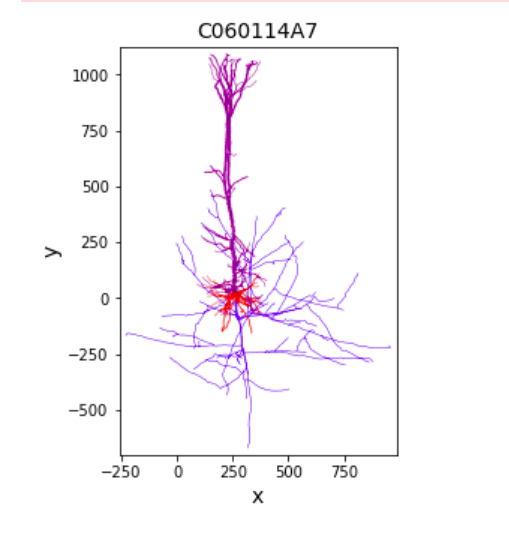
\includegraphics[scale=0.5]{figures/morphology_view.png}
    \caption{This multi-compartment model is spatially extended, so a 2D depiction of its 3D form is warranted.}
  \label{fig:brief_shape}
\end{subfigure}

\begin{subfigure}%{.2\textwidth}
  \centering
    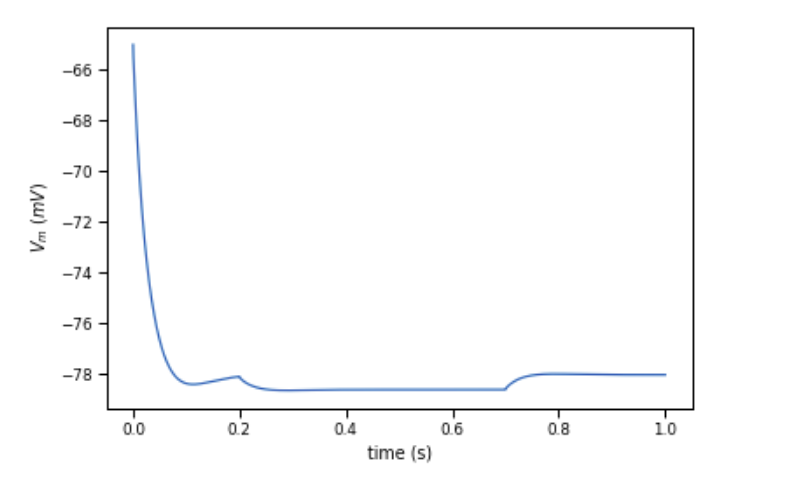
\includegraphics[scale=0.5]{figures/correct_passive_l5pc.png}
    \caption{A current injection value of -$10pA$ is applied to the cell for the duration of $200ms-700ms$}
  \label{fig:passive_properties_fine}
\end{subfigure}
\label{fig:test}
\end{center}
\end{figure}



A test suite was constructed using NeuroElectro for the non specific [cortical regions] layer 4/5 cortex pyramidal cell, and we were able to evaluate this layer 5 PC cells against the criteria of the neuroelectro test suite. Note the unnatural looking brief spike duration of the model cell spike  \ref{fig:brief_shape}. It is possible that the majority neuroelectro experiments on the layer 5 pyramidal cell were conducted under room temperature as opposed to body temperature, as there is evidence that the temperature of cortical tissue modulates spike width \cite{goldin2017temperature}, in particular cooling can contract their spike width

%%
% https://neuroelectro.org/data_table/36261/
%%
% from spike width table: 0.65 ± 0.13	1.04 ± 0.25**	0.51 ± 0.03**	0.59 ± 0.06	0.61 ± 0.03
%%
%



\subsubsection{Optimized Results}
\begin{table}[ht]
\centering
\resizebox{\textwidth}{!}{
\begin{tabular}{lllll}
\toprule
{} & observations &                 predictions &   Z-Scores \\
\midrule
RheobaseTest                   &    213.85 pA &                   213.85 pA &  2.444e-06 \\
InputResistanceTest            &  120.67 Mohm &  183.56713371523054 megaohm &     0.8102 \\
TimeConstantTest               &     15.73 ms &   0.00016898141845179352 ms &     -2.152 \\
CapacitanceTest                &    150.58 pF &    0.0009205428827686333 pF &     -1.078 \\
RestingPotentialTest           &    -68.25 mV &        -71.8621793344104 mV &    -0.5533 \\
InjectedCurrentAPWidthTest     &      1.21 ms &                    2.075 ms &      1.623 \\
InjectedCurrentAPAmplitudeTest &     80.44 mV &        63.31628969975701 mV &     -1.343 \\
InjectedCurrentAPThresholdTest &    -42.74 mV &      -44.863238963316746 mV &    -0.2646 \\
\bottomrule
\end{tabular}}
\caption{observations, predictions and Z-scores pertaining to the NeuronUnit optimized Layer 5 Pyramidal Neuron}
\label{tab:l5pc_table}
\end{table}

Due to computational limitations this model was only run for 
$12$ offspring, and $30$ generation. Actually a minimum of $MU=100$, $NGEN =100$ was prescribed by the scientists who optimized the initial model, however such a large compute job required prohibitive computational resources.


The unoptimized model had statistics:
$(\chi^{2},p_{value})=(13.5609360364, 0.093951963105254)$

The optimized model produced statistics
$(\chi^{2},p_{value})=(6.632440090005973 0.5767576828862497)$

Optimization then clearly improves the model, however, it does not bring the model  biological plausibity.





This can be improved by omitting some of the worst tests, overall, the tests are compromized.



It is worth noting that the layer 5 neocortical pyramidal neuron was very slow to dispatch relative to the reduced models developed in this thesis work. Where as a typical reduced model described here evaluated in the order of $~0.0025 seconds$, this model on average took $5.74$, for a single run and $34.8$ to solve for the models Rheobase, current.

This model was pre-optimized to fit to spike times and F/I mainly, and so it should not necassarily be expected to fit other electrical charactersistics of the cell. Only the rheobase test, and the time constant test seemed to fall within the range of biological plausibility.
None the less, this model remains a useful benchmark for reduced neuronal models.